\scanpage{276}


Détermination d'un sommet (d'un \inserted{2-}polyèdre triangulé) par son étoile.

1) Soient $\inserted{P=}(S,F\subset\unsure{\mathfrak P_3(S)|P_3(S)})$ un 2-polyèdre triangulé connexe, $s,s'\in S$ tels que \deleted{\unsure{s}} l'on ait

\[
s\ne s',\quad\operatorname{Et}(s)=\operatorname{Et}(s').
\]

Alors on a

\[
S=\{s,s'\}\cup\operatorname{Et}(s)
\]

i.e. $P$ s'identifie au double cône sur le $n$-polygône $\operatorname{Et}(s)$ ($n\inserted{=\operatorname{card}\operatorname{Et}(s)}\geq3$).

\figure{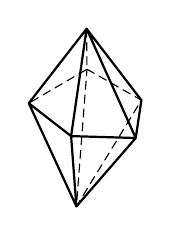
\begin{tikzpicture}[x=.48cm,y=.48cm,line cap=round,line join=round]
\coordinate (N) at (0.22,2.95);\coordinate (S) at (-0.05,-1.75);
\coordinate (L) at (-1.31,.98);\coordinate (F) at (-.19,.11);
\coordinate (R) at (1.52,.06);\coordinate (E) at (1.67,1.06);\coordinate (B) at (.23,1.88);
\draw[thick] (N)--(L)--(F)--(R)--(E)--cycle (N)--(F)--(S)--(R)--(N) (L)--(S);
\draw[densely dashed] (N)--(B)--(L) (B)--(E)--(S)--(B);
\end{tikzpicture}}

\uline{NB} Les deux sommets $s,s'$ sont d'ordre $n$, les autres sommets sont d'ordre 4. Si tous les sommets ont même ordre, on a donc $n=4$, et $P$ est un octaèdre. Dans ce cas, pour que deux sommets aient même étoile, il f. et s. qu'ils soient antipodiques. Dans le cas $n\ne4$, la seule paire de sommets ayant $\unsure{=|\text{m\textsuperscript{me}}}$ étoile est $\{s,s'\}$ (car \deleted{\unsure{que}} s'il y avait une autre \deleted{\unsure{sommet}} telle paire $\{t,t'\}$, \deleted{les} l'ordre de $t,t'$ serait quatre, et $P$ serait un octaèdre, absurde !). Mais dans ce cas, il existe encore un automorphisme unique (qui mérite le nom d'antipodisme ?) \unsure{$u$|$a$|i.e.}\inserted{$\underline a\ne\mathrm{id}$}, tel que pour \deleted{que} $t\in S$, on ait $\operatorname{Et}(t)=\operatorname{Et}(\underline a(t))$ ; cet automorphisme est la transposition de $s,s'$ et l'identité sur $E=\operatorname{Et}(s)=\operatorname{Et}(s')$. Il est involutif, et ses orbites sont les classes pour la relation
% archive sheet number: 275
